%% 
%% Copyright 2019-2024 Elsevier Ltd
%% 
%% This file is part of the 'CAS Bundle'.
%% --------------------------------------
%% 
%% It may be distributed under the conditions of the LaTeX Project Public
%% License, either version 1.3c of this license or (at your option) any
%% later version.  The latest version of this license is in
%%    http://www.latex-project.org/lppl.txt
%% and version 1.3c or later is part of all distributions of LaTeX
%% version 1999/12/01 or later.
%% 
%% The list of all files belonging to the 'CAS Bundle' is
%% given in the file `manifest.txt'.
%% 
%% Template article for cas-sc documentclass for 
%% double column output.

\documentclass[a4paper,fleqn]{cas-sc}

% If the frontmatter runs over more than one page
% use the longmktitle option.

%\documentclass[a4paper,fleqn,longmktitle]{cas-sc}

%\usepackage[numbers]{natbib}
%\usepackage[authoryear]{natbib}
% \usepackage[authoryear,longnamesfirst]{natbib}
\usepackage{subfigure}
\usepackage[hyperref=true,backend=biber,sorting=none,backref=true]{biblatex}
\addbibresource{cas-refs.bib}

%%%Author macros
\def\tsc#1{\csdef{#1}{\textsc{\lowercase{#1}}\xspace}}
\tsc{WGM}
\tsc{QE}
%%%

% Uncomment and use as if needed
%\newtheorem{theorem}{Theorem}
%\newtheorem{lemma}[theorem]{Lemma}
%\newdefinition{rmk}{Remark}
%\newproof{pf}{Proof}
%\newproof{pot}{Proof of Theorem \ref{thm}}

\begin{document}
\let\WriteBookmarks\relax
\def\floatpagepagefraction{1}
\def\textpagefraction{.001}

% Short title
\shorttitle{Holographic dark energy models in {$f(Q,T)$} gravity and cosmic constraint}    

% Short author
\shortauthors{Zhang et~al.}  

% Main title of the paper
\title [mode = title]{Holographic dark energy models in {$f(Q,T)$} gravity and cosmic constraint}  

% Title footnote mark
% eg: \tnotemark[1]
% \tnotemark[1] 

% Title footnote 1.
% eg: \tnotetext[1]{Title footnote text}
% \tnotetext[1]{} 

% First author
%
% Options: Use if required
% eg: \author[1,3]{Author Name}[type=editor,
%       style=chinese,
%       auid=000,
%       bioid=1,
%       prefix=Sir,
%       orcid=0000-0000-0000-0000,
%       facebook=<facebook id>,
%       twitter=<twitter id>,
%       linkedin=<linkedin id>,
%       gplus=<gplus id>]

\author[1,2]{Xuwei Zhang}[orcid=0009-0002-9943-4062]

% Footnote of the first author
% \fnmark[1]
% Email id of the first author
\ead{zhangxuwei@xao.ac.cn}
% URL of the first author
% \ead[url]{}
% Credit authorship
% eg: \credit{Conceptualization of this study, Methodology, Software}
% \credit{}



\author[1,2]{Xiaofeng Yang}[orcid=0000-0000-0000-0000]
% Corresponding author indication
\cormark[1]
% Footnote of the second author
% \fnmark[2]
% Email id of the second author
\ead{yangxiaofeng@xao.ac.cn}
% URL of the second author
% \ead[url]{}
% Credit authorship
% \credit{}

\author[1,3]{Yunliang Ren}[orcid=0000-0002-9659-4581]
% Footnote of the second author
% \fnmark[2]
% Email id of the second author
% \ead{}
% URL of the second author
% \ead[url]{}
% Credit authorship
% \credit{}

\author[1,3]{Shuangnan Chen}[orcid=0009-0001-5887-7652]
% Footnote of the second author
% \fnmark[2]
% Email id of the second author
% \ead{}
% URL of the second author
% \ead[url]{}
% Credit authorship
% \credit{}

\author[1,4]{Yangjun Shi}[orcid=0009-0007-8857-7371]
% Footnote of the second author
% \fnmark[2]
% Email id of the second author
% \ead{}
% URL of the second author
% \ead[url]{}
% Credit authorship
% \credit{}

% Address/affiliation
\affiliation[1]{organization={Xinjiang Astronomical Observatory, Chinese Academy of Sciences},
            addressline={150 Science 1-Street}, 
            city={Urumqi},
%          citysep={}, % Uncomment if no comma needed between city and postcode
            postcode={830011}, 
            % state={},
            country={China}}
% Address/affiliation
\affiliation[2]{organization={School of Astronomy and Space Science, University of Chinese Academy of Sciences},
            addressline={No.19A Yuquan Road},
            city={Beijing},
            postcode={100049},
            % state={},
            country={China}}
% Address/affiliation
\affiliation[3]{organization={School of Physical Science and Technology, Xinjiang University},
            addressline={666 Shenli Street},
            city={Urumqi},
            postcode={830046},
            % state={},
            country={China}}
% Address/affiliation
\affiliation[4]{organization={School of Physics and Astronomy, China West Normal University},
            % addressline={666 Shenli Street},
            city={Nanchong},
            postcode={637002},
            % state={},
            country={China}}


% Here goes the abstract
\begin{abstract}
In this work, we investigate a modified gravity model $ f(Q,T) $ with holographic dark energy. By considering the holographic principle as an extension to cosmology, we explore dark energy as a result of the entanglement entropy of the universe's horizon. We employ the Barrow holographic dark energy model, incorporating quantum corrections, and use the Hubble horizon for the infrared cutoff. Through parameter estimation using MCMC with the latest supernova, BAO, and Hubble data, we find that the model alleviates the Hubble tension and provides consistent results with the standard cosmological model. Additionally, the model successfully describes the accelerated expansion of the universe. Despite the complexity and additional parameters introduced by the model, it offers a promising framework for further exploration of dark energy within modified gravity theories.
\end{abstract}

% Use if graphical abstract is present
%\begin{graphicalabstract}
%\includegraphics{}
%\end{graphicalabstract}

% Research highlights
% \begin{highlights}
% \item 
% \item 
% \item 
% \end{highlights}


% Keywords
% Each keyword is seperated by \sep
\begin{keywords}
Cosmology \sep Dark energy \sep $f(Q,T)$ gravity\sep Observational estimation
\end{keywords}

\maketitle

% Main text
\section{Introduction} \label{sec:intro}

Over the past few decades, a series of major discoveries in cosmology have profoundly reshaped our understanding of the universe. In 1998, the accelerated expansion of the universe was first observed through studies of Type Ia supernovae \cite{perlmutter_discovery_1998, Riess_1998}. This groundbreaking discovery was later confirmed by various other cosmological observations, including measurements of temperature anisotropies and polarization in the cosmic microwave background (CMB) radiation \cite{1992ApJ...396L...1S, 2020Planck}, the peak length scale of baryon acoustic oscillations (BAO) \cite{Eisenstein_2005, 10.1111/j.1365-2966.2011.19592.x}, the study of the large-scale structure (LSS) of the universe \cite{Dodelson_2002, Percival_2007}, and direct measurements of the Hubble parameter using cosmic chronometers \cite{Daniel_Stern_2010, Moresco_2015}. These observations point to the existence of a mysterious form of energy, referred to as dark energy (DE), which is characterized by negative pressure and an increasing density. Dark energy is believed to be responsible for driving the accelerated expansion of the universe, acting like anti-gravity, although its precise nature remains unknown.

This mysterious energy is thought to account for approximately 70\% of the total energy content of the universe \cite{PhysRevD.37.3406, PhysRevD.63.103510, 10.1143/PTP.106.929}. For such accelerated expansion to occur, dark energy must produce a repulsive gravitational effect that permeates the entire observable universe. Ordinary baryonic matter, however, does not exhibit the properties required to explain this phenomenon, nor can it account for such a significant portion of the universe's energy budget. As a result, researchers have proposed and studied a variety of alternative theories and models to explore the nature of dark energy and the cosmic acceleration it causes \cite{10.1093/oso/9780198526827.001.0001}.

The simplest and most widely accepted theory is $\Lambda \text{CDM}$ model, where $\Lambda$ means cosmological constant predicted by Einstein \cite{Carroll_2001}.
Based on $\Lambda \text{CDM}$ model, the lastest observations suggest that our universe consists of 68.3\% dark energy, 26.8\% cold dark matter and 4.9\% ordinary matter \cite{2020Planck}. However, this model is not free from problems and the problems it is facing are cosmic coincidence, fine-tuning and the Hubble tension, a discrepancy between the value of the Hubble constant $H_0$ inferred from the CMB by the Planck satellite and that obtained from local measurements using Type Ia supernovae—has sparked significant debate. 

Another interesting attempt is to deviate from general ralativity toward a modified form (detailed research progress can be reviewid in \cite{Clifton_2012}). These theories assume that general relativity not work in large scale requiring a modification in action rather than standard Einstein-Hilbert action. The most well-known is $f(R)$ gravity which replaces the Ricci scalar $R$ in the action by a general function $f(R)$ \cite{1970MNRAS.150....1B}. The $f(G)$ gravity theory is also a modified theory of gravity that introduces a correction to the Gauss–Bonnet (GB) term $G$, allowing it to be arbitrary function $f(G)$ rather than remaining a constant \cite{NOJIRI20051,NOJIRI_2007}. Another modified theory of gravity $f(T)$ extends the teleparallel equivalent of General Relativity (TEGR). It replaces the curvature scalar $R$ in action with the torsion scalar $T$, derived from the Weitzenböck connection. Also shows some interpretations for the accelerating phases of our Universe \cite{Cai_2016,Bengochea_2009}. $f(Q)$ is generalized symmetric teleparallel gravity, with curvature and torsion both being zero, which is inspired by Weyl and Einstein's trial to unify electromagenetic and gravity. The geometric properties of gravity are described by "non-metricity". That is, the covariant derivative of the metric tensor is no longer zero (some detailed information can be found in review \cite{HEISENBERG20241}). Harko et al. have proposed a new theory known as $f (R, T )$ gravity, where $R$ stands for the Ricci scalar and $T$ denotes the trace of energy-momentum tensor which presents a non-minimum coupling between geometry and matter \cite{PhysRevD.84.024020}. Similar theories are introduced,$f(R,G)$ gravity proposed by Bamba et al. \cite{Bamba2009FinitetimeFS}; $f(Q,T)$ proposed by Xu et al. \cite{Xu_2019}; $f(Q,C)$ gravity \cite{De_2024}; $f(\mathcal{T},T)$ proposed by \cite{Harko_2014}; $f(T,B)$ gravity \cite{Bahamonde_2015,Bahamonde_2017}; $f(R,T^2)$ proposed by Katirci et al. \cite{Kat_rc__2014}, etc.

Holographic dark energy is an famous alternative theory for the interpretation of dark energy, originating from the holographic principle proposed by 't Hooft \cite{hooft2009dimensionalreductionquantumgravity}. Cohen et al. introduced the "UV-IR" relationship, highlighting that in effective quantum field theory, a system of size $L$ has its entropy and energy constrained by the Bekenstein entropy bound and black hole mass, respectively. This implies that quantum field theory is limited to describing low-energy physics outside black holes \cite{cohen_effective_1999}. After that, Li et al. proposed that the infrared cut-off relevant to the dark energy is the size of the event horizon and obtained the dark energy density can be described as $\rho_\text{de}=3c^2 M_p^2 R_h^2$ where $R_h$ is future horizon of our universe \cite{LI20041}. Although choose Hubble cut-off is a natural thought, but Hsu found it might lead to wrong state equation and be strongly disfavored by observational data \cite{Hsu_2004}.

Various attempts to reconstruct or discuss HDE in modified gravity have been completed by several authors. Wu and zhu reconstructed HDE in $f(R) $ gravity \cite{wu_reconstructing_2008}. Shaikh et al. discussed HDE in $f (G)$ gravity with Bianchi type 1 model \cite{shaikh_holographic_2020}. Zubair et al. reconstructed Tsallis holographic dark energy models in modified $f(T, B)$ gravity \cite{zubair_reconciling_2021}. Sharif et al. studied the cosmological evolution of HDE in $f(\mathcal{G},T)$ gravity \cite{sharif_cosmic_2019} and Alam et al. investigated Renyi HDE in the same gravity \cite{alam_renyi_2023}. Myrzakulov et al. reconstructed Barrow HDE in $f(Q,T)$ gravity \cite{myrzakulov_barrow_2024}. Singh et al. and Devi et al. discussed HDE models respectively in $f(R,T)$ gravity and take cosmic constraint \cite{singh_statefinder_2016,devi_barrow_2024}.

In this article, we assume that our universe is described by $ f(Q,T) $ gravity, with HDE as one component of the fluid. In Section \ref{sec:mg}, we briefly introduce non-Riemannian geometry and $f(Q,T)$ gravity. In Section \ref{sec:solution}, we incorporate HDE into the model and derive the solution. Section \ref{sec:data} presents the data and methods used to obtain constraints. In Section \ref{sec:result}, we analyze the results and investigate the evolution of the models. Finally, Section \ref{sec:conclusion} provides a brief conclusion.

\section{$f(Q,T)$ gravity theory}\label{sec:mg}

Weyl in 1918 introduced an extension of Riemannian geometry, using a non-metricity tensor $Q_{\alpha \mu \nu}=\nabla_\alpha g_{\mu \nu}=-w_\alpha g_{\mu \nu}$, which describes how the length of a vector changes during parallel transport where $w_\alpha$ coincides with those of the electromagnetic potentials \cite{Weyl:1918ib}. Weyl geometry can also be extended to so-called Weyl-Cartan geometry by considering the torsion of spacetime \cite{Xu_2019}.

In Weyl-Cartan geometry, a connection
can be decomposed into three independent parts: the Christoffel symbol $\hat{\Gamma}^\alpha_{\ \mu \nu}$, the contortion tensor $K^\alpha_{\ \mu \nu}$ and the disformation tensor $L^\alpha_{\ \mu \nu}$, so that the general affine connection can be expressed as \cite{J_rv_2018}
\begin{equation}
    \Gamma^\alpha_{\ \mu \nu}=\hat{\Gamma}^\alpha_{\ \mu \nu}+K^{\alpha}{}_{\mu \nu}+L^\alpha{}_{\mu \nu}
\end{equation}
whereas
\begin{align}
    \hat{\Gamma}^\alpha{}_{\mu \nu}& =\frac{1}{2}g^{\alpha \beta}(\partial_\mu g_{\beta \nu}+\partial_\nu g_{\beta \mu}-\partial_\beta g_{\mu \nu}) \\
    K^{\alpha }{}_{\mu \nu }& = \frac{1}{2}T^{\alpha }{}_{\mu \nu }+T_{(\mu}{}^{\alpha }{}_{\nu )} \\
    L^{\alpha}{}_{\mu\nu}& = \frac{1}{2}Q^{\alpha}_{}{\mu\nu}-Q_{(\mu}{}^{\alpha }{}_{\nu)}
\end{align}
are the standard Levi-civita connection of metric $g_{\mu \nu}$, contortion and disformation tensors respectively.
In the above definitions, the torsion tensors and the non-metric tensor are introduced as follow
\begin{align}
Q_{\rho \mu\nu} &\equiv \nabla_{\rho} g_{\mu\nu} = \partial_\rho g_{\mu\nu} - \Gamma^\beta{}_{\rho \mu} g_{\beta\nu} - \Gamma^\beta{}_{\rho\nu} g_{\mu\beta}\\
T^{\alpha}{}_{\mu\nu} &\equiv 2\Gamma^{\alpha}{}_{[\mu\nu]} =\Gamma^{\alpha}{}_{\mu\nu}-\Gamma^{\alpha}{}_{\nu\mu}
\end{align}
The non-metric tensor has two independent traces, namely $Q_{\mu}=Q_{\mu}{}^{\alpha}{}_{\alpha}$ and $\tilde{Q}^{\mu}=Q_{\alpha}{}^{\mu \alpha}$, so we can get quadratic non-metricity scalar as
\begin{equation}
    Q=\dfrac{1}{4}Q_{\alpha\beta\mu}Q^{\alpha\beta\mu}-\dfrac{1}{2}Q_{\alpha\beta\mu}Q^{\beta\mu\alpha}-\dfrac{1}{4}Q_{\alpha}Q^{\alpha}+\dfrac{1}{2}Q_{\alpha}\tilde{Q}^\alpha\label{Qscalar} 
\end{equation} 

We consider the general form of the Einstein-Hilbert action for the $f(Q,T)$ gravity in the unit $8\pi G=1$
\begin{equation}
S=\int(\frac{1}{2}f(Q,T)+\mathcal{L}_m) \sqrt{-g}  d^4x \label{action}
\end{equation}
where $f$ is an arbitrary function of the non-metricity , $\mathcal{L}_m$ is known as matter Lagrangian, $g=\det (g_{\mu \nu})$ denotes determinant of metric tensor, and $T=g^{\mu \nu}T_{\mu \nu}$ is the trace of the matter-energy-momentum tensor, where $T_{\mu \nu}$ is defined as
\begin{equation}
    T_{\mu \nu}=-\frac{2}{\sqrt{-g}}\frac{\delta(\sqrt{-g}\mathcal{L}_m)}{\delta g^{\mu \nu}}
\end{equation}
Vary the action \eqref{action} with respect to the metric tensor $g_{\mu\nu}$ we can get
\begin{align}
\delta S&=\int \left(\frac{1}{2} \delta[f(Q,T) \sqrt{-g}]+\delta(\mathcal{L}_m \sqrt{-g})\right)d^4x \\
&= \int \frac{1}{2}\left(-\frac{1}{2}f g_{\mu\nu}\sqrt{-g}\delta g^{\mu\nu}+f_Q \sqrt{-g} \delta Q+f_T \sqrt{-g}\delta T -\frac{1}{2}T_{\mu \nu}\sqrt{-g}\delta g^{\mu\nu}\right)d^4x
\end{align}
In analogy to studies on torsionless $f(R)$ gravity and curvature-free $f(T)$ gravity, we can generalize the gravity to theories containing an arbitrary function of the non-metricity scalar i.e. $f(Q,T)$. Therefore, we consider the following action
\begin{equation}
-\frac{2}{\sqrt{-g}}\nabla_\alpha(f_Q \sqrt{-g}P^\alpha_{\ \ \mu \nu})-\frac{1}{2}f g_{\mu \nu}+f_T(T_{\mu \nu}+\Theta_{\mu \nu})-f_Q(P_{\mu \alpha \beta}Q^\nu_{\ \ \alpha \beta}-2Q^{\alpha \beta}_{\ \ \ \ \mu}P_{\alpha \beta \nu})=T_{\mu \nu}\label{FieldEq}
\end{equation}
Where tensor $\Theta_{\mu \nu}$ are defined as $g^{\alpha\beta}\delta T_{\alpha\beta}/{\delta g^{\mu\nu}}$ and $P^{\alpha}_{\mu\nu}$ is the super-potential of the model (detailed discussion found in \cite{Xu_2019}). In the case of a globally vanishing affine connections, the non-metricity tensor depends on the metric only and Einstein's GR action is recovered. This occurs under the choice of the coincidence gauge, in which the origin of spacetime and that of the tangent space coincide. 

Assuming that the Universe is described by the isotropic, homogeneous and spatially flat Friedmann-Lemaitre-Robertson-Walker (FLRW) spacetime, given by as line element
\begin{equation}
    ds^2=-N^2(t)dt^2+a^2(t)\delta_{ij} dx^i dx^j\label{FLRW}
\end{equation}
where $a(t)$ is the cosmic scale factor
used to define the Hubble expansion rate $H=\dot{a}/a$ and the lapse function $N(t)$ used to define dilation rates $\tilde{T}=\dot{N}/N$ (for standard case $N(t)=1$). To derive Friedmann equations describing the cosmological evolution, we assume that the matter content of the Universe consists of a perfect fluid, whose  energy-momentum tensor is given by $T^{\mu}_\nu=\text{diag}(-\rho,p,p,p)$ and tensor $\Theta^{\mu}_\nu$ is expressed as $\text{diag}(2\rho+p,-p,-p,-p)$. Then use the line element \eqref{FLRW} and field equation \eqref{FieldEq}, we can get Friedmann equations
\begin{align}
    \rho &=\frac{f}{2}-6f_Q H^2-\frac{2f_T}{1+f_T}(\dot{f}_QH+f_Q \dot{H})\label{Fr1} \\
    p &=-\frac{f}{2}+6f_Q H^2+2(\dot{f}_QH+f_Q \dot{H})\label{Fr2} 
\end{align}
where $f(Q,T)$ is simplified to $f$, and $f_Q=\partial f/\partial Q$, $f_T=\partial f/\partial T$, $\dot{f}_Q=\partial f_Q/\partial t$. In the coincident gauge with $\Gamma^{\alpha}_{\mu\nu}=0$, the usage of Eq. \eqref{Qscalar} and the line element \eqref{FLRW}, there exists following relationship (The detailed derivation can be found in the appendix of \cite{Xu_2019} and \cite{lu2019cosmologysymmetricteleparallelgravity})
\begin{equation}
    Q=6H(t)^2
\end{equation}

The equation of state (EoS) parameter is given by
\begin{equation}
    w=\frac{p}{\rho}=-1+\frac{4 f_Q H+f_Q \dot{H}}{(1+f_T)(f-12f_QH^2)-4 f_T(\dot{f}_QH+f_Q \dot{H})},
\end{equation}
where $\rho$ and $p$ denote the total energy density and pressure of the universe. Since we mainly focus in the late universe, the contribution of radiation can be ignored, so we only care about baryonic matter and holographic dark energy fluid,
\begin{equation}
    \rho=\rho_m+\rho_\text{de}, \quad p=p_m+p_\text{de}
\end{equation}
Effective component parameter can be derived from Eq. \eqref{Fr1}\eqref{Fr2} as
\begin{align}
    \rho_{\text{eff}}&=3H^2=\frac{f}{4f_Q}-\frac{1}{2f_Q}[(1+f_T)\rho+f_T p] \label{F1}\\
    -p_{\text{eff}}&=2\dot{H}+3H^2=\frac{f}{4f_Q}-\frac{2\dot{f}_Q H}{f_Q}+\frac{1}{2f_Q}[(1+f_T)\rho +(2+f_T)p] \label{F2}
\end{align}
The two equations describe the total effective energy density \(\rho_{\text{eff}}\) and the total effective pressure \(p_{\text{eff}}\), reflecting the combined effects of all ideal fluid components and the modified gravity. The term \(\frac{f}{4f_Q}\) represents the contribution from modified gravity, while the latter term accounts for the contributions from various fluid components. However, unlike the standard Friedmann equations, there are correction coefficients \(f_T\) and \(f_Q\) that represent interaction modifications. The effective parameters satisfy the conservation equation, but the individual components do not as
\begin{equation}
    \dot{\rho_{\text{eff}}}+3H(\rho_{\text{eff}}+p_\text{eff})=0
\end{equation}
Furthermore, the effective EoS using Eq.\eqref{F1}\eqref{F2} can be written as
\begin{equation}
    w_{\text{eff}}=\frac{p_{\text{eff}}}{\rho_{\text{eff}}} = \frac{-2\dot{H}-3H^2}{3H^2}= -\frac{f - 8\dot{f}_Q H + 2[(1 + f_T)\rho + (2 + f_T)p]}{f - 2[(1 + f_T)\rho + f_T p]}
\end{equation}
It defines the various components of the universe (such as dark energy, dark matter, radiation and ordinary matter and even modified gravity) as a whole, describes the relationship between the pressure and energy density of the total effective fluid, and the expansion of the universe is accelerated when $w_\text{eff}<-1/3$.

\section{Cosmic solutions with holographic dark energy}\label{sec:solution}

The holographic principle sets an upper limit on the entropy of the universe.  In the HDE model, the energy density of dark energy is typically expressed as (\cite{LI20041})
\begin{equation}
    \rho_\text{de} = 3c^2 M_p^2 L^{-2}
\end{equation}
where $L$ is the characteristic length scale of the universe, and $c$ is free parameter, $M_p$ denotes planck mass here we set it as 1. The Hubble horizon is considered the simplest option.  In addition, the particle horizon $L_p$ or the future event horizon $L_F$ are also considered reasonable options. Consider a simple case, the HDE energy density in Hubble cut-off can be described as 
\begin{equation}
    \rho_{de}=3c^2 H(t)^2 \label{HDE}
\end{equation}
Another HDE model called barrow holographic dark energy (BHDE) generalizes holographic entropy that arises from quantum-gravitational effects which deform the black-hole surface by giving it an intricate, fractal form . In this case, the HDE energy density can be define as
\begin{equation}
    \rho_{de}=3c^2 H(t)^{2-\Delta}\label{BHDEdef}
\end{equation}
here a new exponent $\Delta$ quantifies the quantum-gravitational deformation, with $\Delta=0$ coming back to the standard Bekenstein-Hawking entropy, and with $\Delta=1$ corresponding to the most intricate and fractal structure \cite{PhysRevD.102.123525}.

In order to incorporate holographic dark energy in the modified gravitational universe, we consider a simple form of $f$ 
\begin{equation}
    f(Q,T)=m Q^n+\alpha T
\end{equation}
where $Q=6H^2$, $T=-\rho+3p$, $m$, $n$ and $\alpha$ are constants. So that we can derive 
\begin{equation}
    f_Q= mn Q^{n-1}=mn 6^{n-1}H^{2n-2},\  f_T=\alpha,\ \dot{f}_Q=2 mn(n-1)6^{n-1}H^{2n-3}\dot{H}
\end{equation}


We also introduce the deceleration factor, which describes the acceleration or deceleration of the late universe depending upon its value, is defined as
\begin{equation}
    q=\frac{d}{dt}\frac{1}{H}-1=-\frac{\ddot{a}a}{\dot{a}^2}=-\frac{\dot{H}}{H^2}-1=(1+z)\frac{1}{H(z)}\frac{dH(z)}{dz}-1   
\end{equation}
In order to understand the characteristic properties of the dark energy and more easier to get a analytical solution, we need to parameterize EoS of HDE as a constant parameter
\begin{equation}
    w_\text{de}=\frac{p_\text{de}}{\rho_\text{de}}
\end{equation}
Use Eq.\eqref{F1} and \eqref{F2} we can solve the energy density of fluid component in field equation
\begin{align}
    \rho_\text{de}&= \frac{m (2 n-1) \left(6H(t)^2\right)^{n-1} \left((3 \alpha +2) n H'(t)+3 (\alpha +1) H(t)^2\right)}{\left(2 \alpha ^2+3 \alpha +1\right) w_\text{de}} \label{RD}\\
    \rho_m&= \frac{m (2 n-1) \left(6H(t)^2\right)^{n-1} \left(n (\alpha  (w_\text{de}-3)-2) H'(t)-3 (\alpha +1) (w_\text{de}+1) H(t)^2\right)}{\left(2 \alpha ^2+3 \alpha +1\right) w_\text{de}}\label{RM}
\end{align}
This is a second order differential equation and it depends on t. In order to get cosmological solution, there is also a simple relation between $H(t)$ and $H(z)$
\begin{equation}
    \dot{H}(t)=\frac{d}{dt}H(t)=-\frac{d H(z)}{dz}H(z)(1+z)\label{HR}
\end{equation}
Combine Eq.~\eqref{BHDEdef}\eqref{RD} and relation \eqref{HR}, we can get the equation follows
\begin{equation}
    3 c^2 H(z)^{2-\Delta}=\frac{m 6^{n-1} (2 n-1) \left(H(z)^2\right)^{n-1} \left(3 (\alpha +1) H(z)^2-(3 \alpha +2) n (z+1) H(z) H'(z)\right)}{\left(2 \alpha ^2+3 \alpha +1\right) {w_\text{de}}}
\end{equation}
% We first not consider non-minimum coupling between geometry and matter assuming that $\alpha=0$, so that we don't need to talk the dynamic tensor coupling terms $T$. To get an analytic form, we also assume that $n=1$, so we can get
% \begin{equation}
%     H(z) = H_0  (1+z)^{\frac{3}{2}-\frac{3 c^2 w_\text{de}}{2 m}}
% \end{equation}

% \begin{equation}
%     H(z)= H_0(z+1)^{3/2}-c^2 w_\text{de}((1+z)^{3/2}-1)\frac{1}{m}
% \end{equation}
In principle, we can get the form of $H(z)$ through the solution of above differential equation. However, solving higher-order differential equations analytically is difficult. So we consider $n=1$ and $\Delta=0$ firstly to simplify calculation and set the initial condition $H(z=0)=H_0$ which denotes value of the Hubble parameter at present, get analytically solution as follow
\begin{equation}
    H(z)= H_0 (1+z)^{\frac{3 (1+\alpha) \left(m-c^2 w_\text{de}(1+2\alpha)\right)}{m(2+3\alpha)}}
\end{equation}
We thus obtain the power-law evolution of the Universe which avoids the big-bang singularity similar to the $f(R,T)$ situation in \cite{singhStatefinderDiagnosisHolographic2016}. In this case, the deceleration factor is
\begin{equation}
    q = -1+\frac{3 (\alpha +1) \left(m-(2 \alpha +1) c^2 w_\text{de}\right)}{(3 \alpha +2) m}
\end{equation}
Here we have a constant deceleration factor depending on the parameter. When we select a particular parameter value, it will show acceleration or deceleration characteristics. If $q<0$, it will show the characteristics of accelerated expansion. However, since the deceleration factor and effective EOS is time independent, there is no phase transition in such a universe. So we can use Eq. \eqref{BHDEdef} to obtain a tighter UV limit, if we set $\Delta=1$ we can get 
\begin{equation}
    H(z)= H_0 (1+z)^{\frac{3 (\alpha +1)}{3\alpha +2}}-(1+2 \alpha) c^2 w_{de} \left((1+z)^{\frac{3 (\alpha +1)}{3\alpha +2}}-1\right)\frac{1}{m}
\end{equation}
In this case, the deceleration factor is
\begin{equation}
    q=\frac{(2 \alpha +1) c^2 w_\text{de} \left(3 \alpha +(z+1)^{\frac{3 (\alpha +1)}{3 \alpha +2}}+2\right)-H_0 m (z+1)^{\frac{3 (\alpha +1)}{3 \alpha +2}}}{(3 \alpha +2) \left((2 \alpha +1) c^2 w_\text{de} \left((z+1)^{\frac{3 (\alpha +1)}{3 \alpha +2}}-1\right)-H_0 m (z+1)^{\frac{3 (\alpha +1)}{3 \alpha +2}}\right)}
\end{equation}
And if we set $\Delta=0.5$, we can also get a solution analytically as follow
\begin{equation}
    H(z)= \left(2 \alpha  c^2 w_\text{de}+c^2 w_\text{de}+(1+z)^{\frac{3 (\alpha +1)}{6 \alpha +4}}\sqrt{2 \sqrt{(2 \alpha +1)^2 c^4 H_0} m^2 \text{wde}^2+c^4 (2 \alpha  w_\text{de}+w_\text{de})^2+H_0 m^2}\right)^2 \frac{1}{m^2}
\end{equation}
In this case, the deceleration factor and effective EOS is also approaching a constant value, similar to the situation of $\Delta = 0$.
However, in some other situation, if $n \neq 1$ or $\Delta \neq 1,0.5$, higher-order differential equations are difficult to solve analytically, so we can only obtain numerical solutions through complex machine computing. We also consider the case where $\alpha=1$ that reduces it to the minimum matter-energy-momentum tensor coupling.

For comparison in the parameter estimates below, we also consider the case of the standard $\Lambda$CDM model
\begin{equation}
    H(z)=H_0\sqrt{\Omega_m(1+z)^3+\Omega_\Lambda}
\end{equation}
where   $\Omega_m=\rho_{m0}/3H_0^2$ is the matter density parameter, and $ \Omega_\Lambda=\rho_{\text{de}0}/3H_0^2$ is the dark energy density parameter. This model assumes that the universe is composed of matter and a cosmological constant $\Lambda$ with no additional exotic components.


\section{Observational data and methodology}\label{sec:data}


\begin{table}
    \begin{center}
    \caption{BAO dataset used in the study, referenced from \cite{luongoDarkEnergyReconstructions2024}. The table includes data from the 6dFGS survey \cite{Beutler_2011}, SDSS survey \cite{PhysRevD.103.083533}, and DESI 2024 BAO data \cite{desicollaboration2024desi2024vicosmological}. The table provides effective redshifts $ z_\text{eff} $, along with measurements of the ratio $ D_{\rm M}/r_{\rm d} $, $ D_{\rm H}/r_{\rm d} $, and $ D_{\rm V}/r_{\rm d} $ respectively.}
    \label{tab:baodata}
    \begin{tabular}{lcccc}
    \toprule
    Survey          & $z_\text{eff}$ & $D_{\rm M}/r_{\rm d}$ & $D_{\rm H}/r_{\rm d}$ & $D_{\rm V}/r_{\rm d}$\\
    \midrule
    6dFGS		    & $0.106$	& & & $2.98\pm0.13$ \\
    \midrule
    SDSS MGS 		& $0.15$	& & & $4.51\pm0.14$ \\
    SDSS DR12		& $0.38$    & $10.27\pm0.15$ & $24.89\pm 0.58$ & \\
    SDSS DR12		& $0.51$    & $13.38\pm0.18$ & $22.43\pm 0.48$ & \\
    SDSS DR16 LRG	& $0.70$    & $17.65\pm0.30$ & $19.78\pm0.46$ & \\
    SDSS DR16 ELG	& $0.85$	& $19.50\pm1.00$ & $19.60\pm2.10$ & \\
    SDSS DR16 QSO	& $1.48$    & $30.21\pm0.79$ & $13.23\pm0.47$ & \\
    SDSS DR16 Ly$\alpha$-Ly$\alpha$& $2.33$     & $37.60\pm1.90$& $8.93\pm0.28$ & \\
    SDSS DR16 Ly$\alpha$-QSO	& $2.33$ & $37.30\pm1.70$& $9.08\pm0.34$ & \\
    \midrule
    DESI BGS 		& $0.30$    & & & $7.93\pm0.15$ \\
    DESI LRG1	 	& $0.51$ 	& $13.62\pm0.25$ & $20.98\pm0.61$ & \\
    DESI LRG2       & $0.71$ 	& $16.85\pm0.32$ & $20.08\pm0.60 $& \\
    DESI LRG+ELG    & $0.93$    & $21.71\pm0.28$ & $17.88\pm0.35$ & \\
    DESI ELG        & $1.32$    & $27.79\pm0.69$ & $13.82\pm0.42$ & \\
    DESI QSO		& $1.49$	& & & $26.07\pm0.67$ \\
    DESI Ly$\alpha$-QSO & $2.33$ 	& $39.71\pm0.94$ & $8.52\pm0.17$ & \\
    \bottomrule
    \end{tabular}
    \end{center}
\end{table}

\begin{figure}
    \centering
    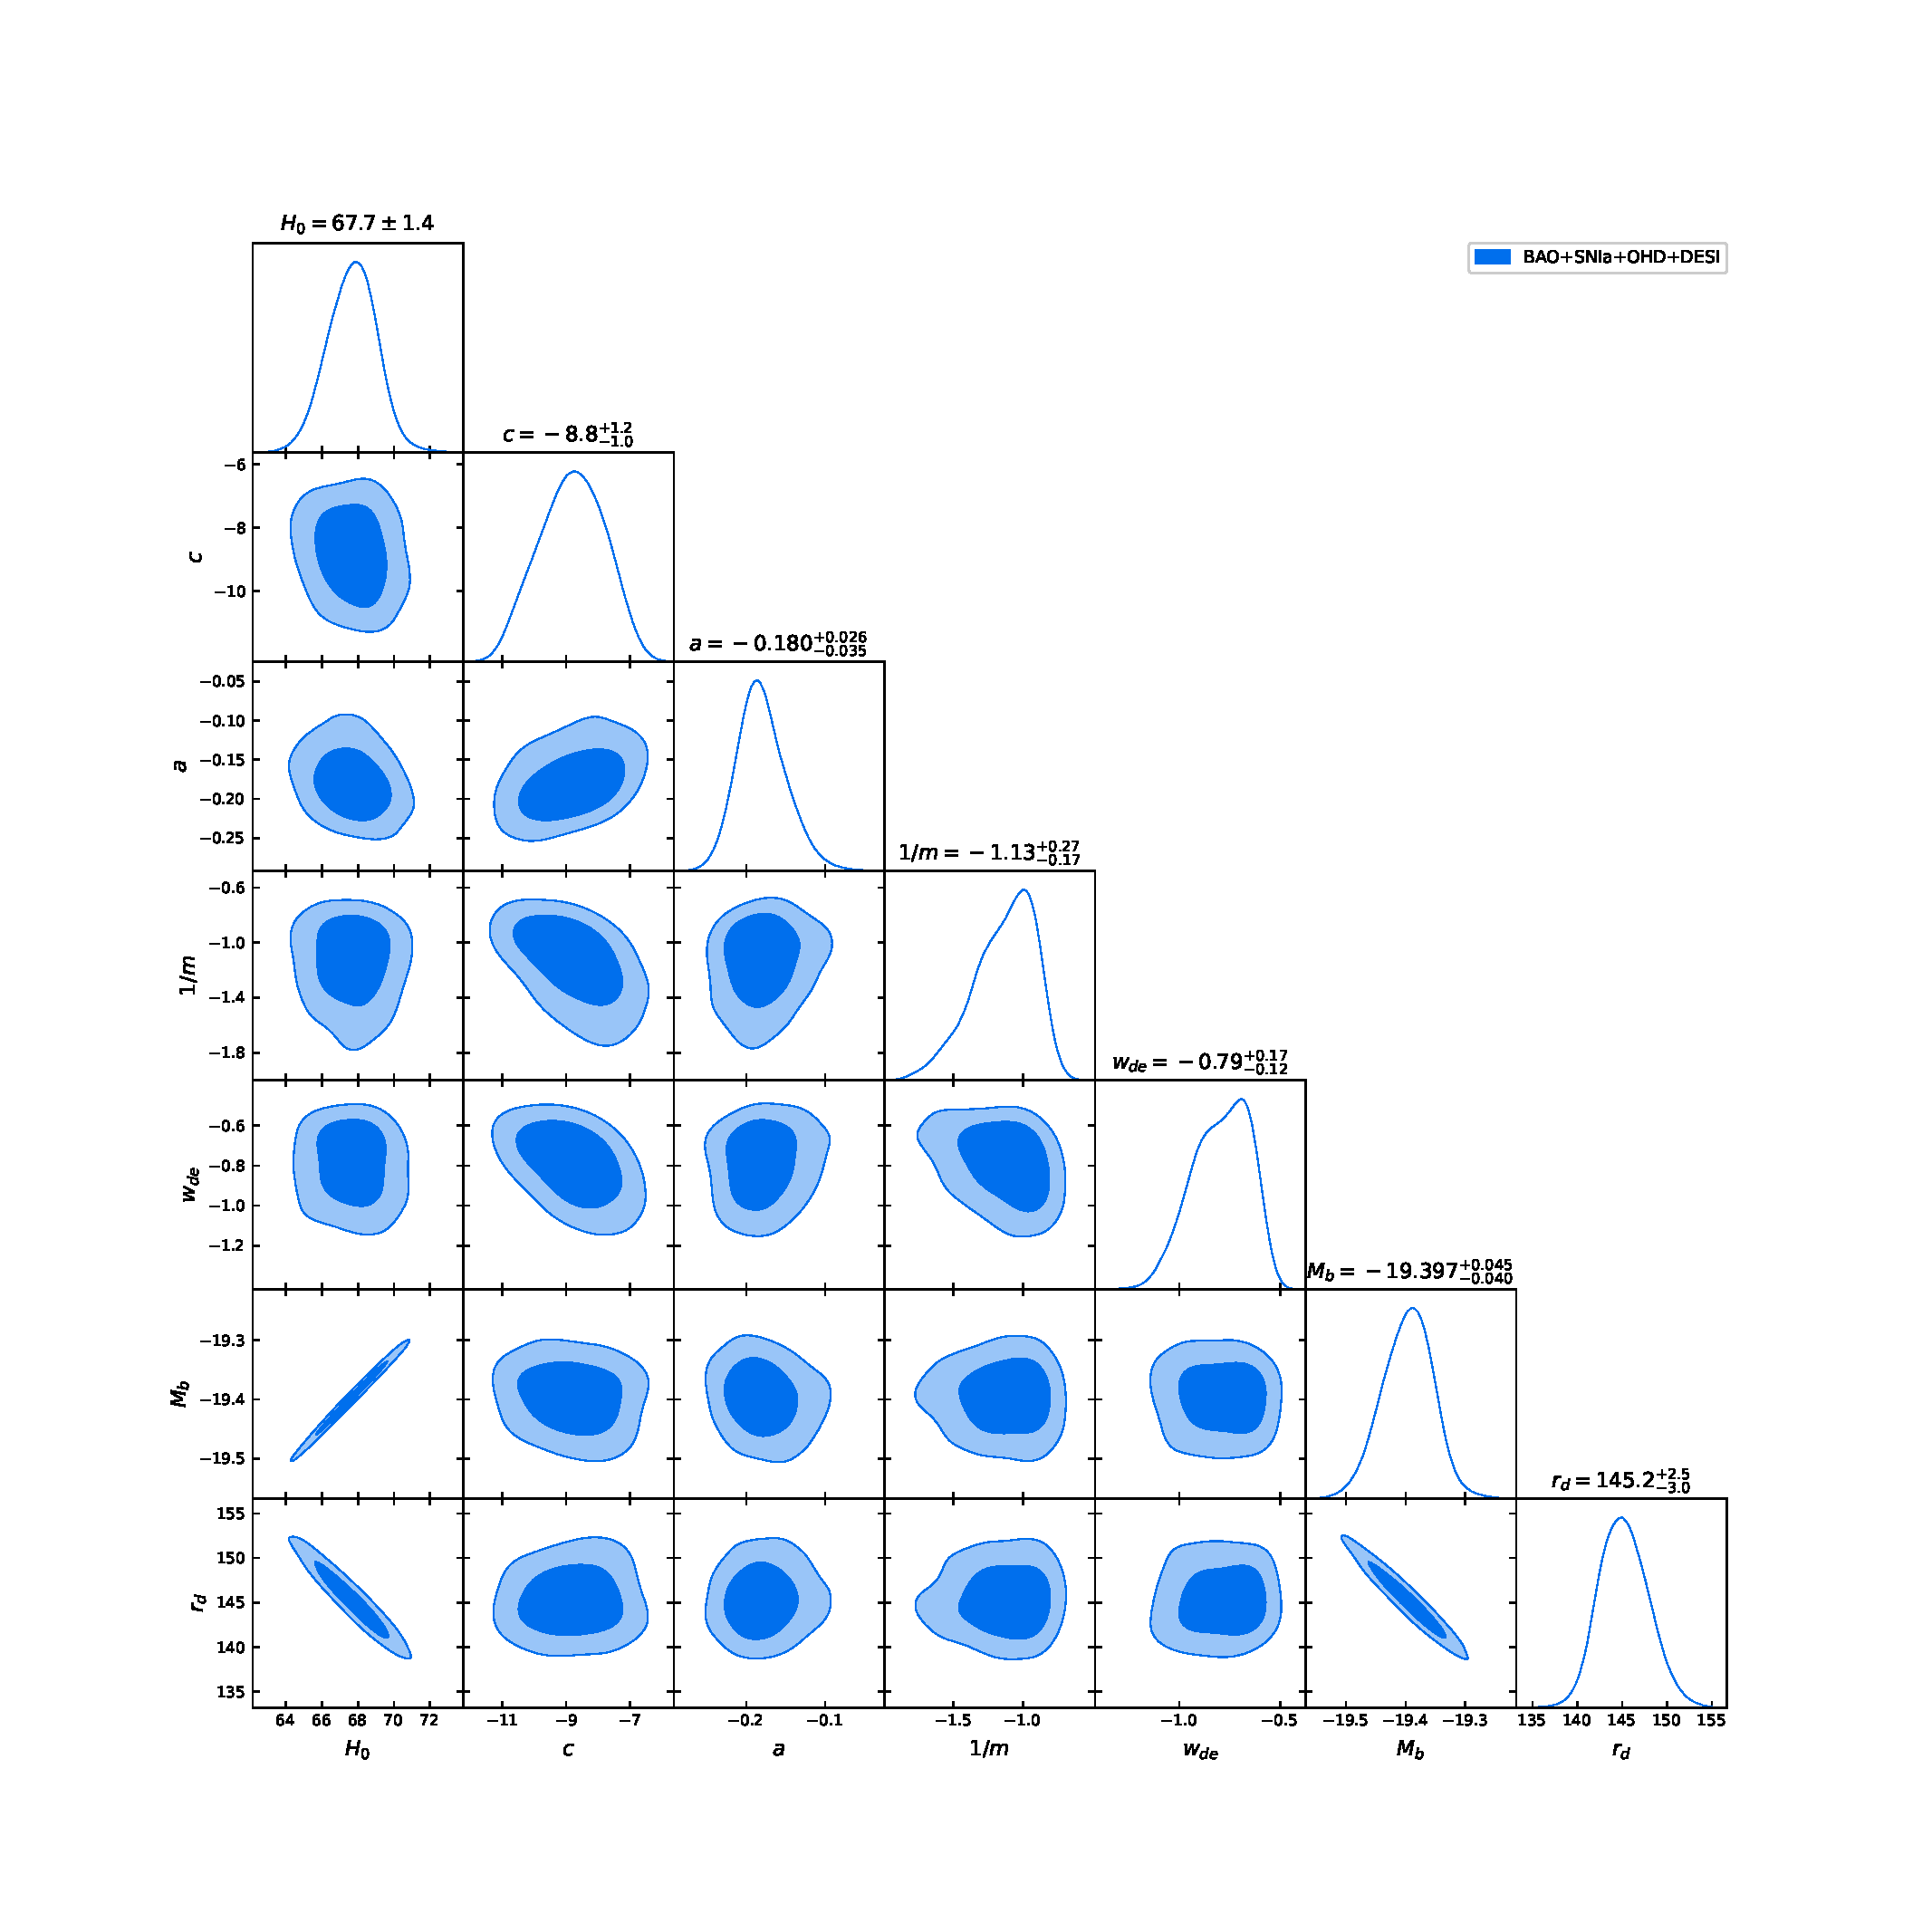
\includegraphics[width=1\linewidth]{./pic/getdist.eps}
    \caption{\label{Fig:constraint} The 1$\sigma$ and 2$\sigma$ confidence contours and the 1D posterior distributions obtained from MCMC constraint of HDE in $f(Q,T)$ gravity using BAO+SNIa+OHD+DESI data. Here we show the results of only one of the model parameter estimates, additional results can be found in code.}
\end{figure}

In this work, we estimate the cosmological parameters of the model by employing a Markov Chain Monte Carlo (MCMC) method based on the minimization of the chi-square function, $\chi^2$ \cite{Padilla_2021}\footnote{The code we used can be found in \url{https://github.com/suiranruofeng/HDE-in-Modified-Gravity}}. The chi-square function is given by:
\begin{equation}
\chi^2 = \sum_i \left(\frac{D_i - T_i(\mathbf{\theta})}{\sigma_i}\right)^2,
\end{equation}
where $D_i$ represents the $i$-th data point, $T_i(\mathbf{\theta})$ is the theoretical prediction for the corresponding quantity, and $\sigma_i$ is the error associated with the $i$-th data point. Here, $\mathbf{\theta}$ denotes the vector of model parameters. To complete the parameter constraints, we utilize the Python package \texttt{emcee} \cite{emcee}, a user-friendly MCMC implementation well-suited for cosmological data analysis.


For our analysis, we combine three independent observational datasets:

1. Baryon Acoustic Oscillations (BAO): The BAO measurements provide a standard ruler for distance measurements in the universe. We use the data from the SDSS Baryon Oscillation Spectroscopic Survey (BOSS)  \cite{PhysRevD.103.083533}, Dark Energy Spectroscopic Instrument (DESI) first year data \cite{desicollaboration2024desi2024vicosmological} and 6dF Galaxy Survey (6dFGS) to constrain the cosmological parameters \cite{Beutler_2011}. The comoving horizon distance, the transverse comoving distance
and the volume-averaged distance ombineing line-of-sight and transverse distances defined as follow
\begin{align}
    D_H&=\frac{c}{H(z)} \\
    D_M&=\frac{d_L}{1+z}\\
    D_V&=\left[\frac{cz}{H(z)}\right]^{1/3}\left[\frac{d_L}{1+z}\right]^{2/3}
\end{align}
Where $d_L$ is the luminosity distance (defined in Eq.~\eqref{dL}). When scaled by the sound horizon at the drag epoch $r_d$ , ratios such as $D_H/r_d$, $D_M/r_d$, and $D_V/r_d$ serve as important observables for constraining cosmological models and testing the standard model of cosmology.



2. Cosmic chronometers (CC) Data : The Hubble parameter measurements, known as the chronometers data, provide independent estimates of the Hubble parameter $H(z)$ at various redshifts. These data serve as an important probe of the expansion rate of the universe. We choose the dataset from \cite{Favale_2023} which includes 32 CC data points incorporating both the statistical and systematic errors within the redshift range of $0.07 < z < 1.965$.

3. Type Ia Supernovae (SNIa) Data: Type Ia supernovae (SNIa) are considered standard candles because When the light curve reaches its maximum, the absolute luminosity is almost the same. The distance modulus $\mu$ can be obtained according to the following formula
\begin{equation}
    \mu_{obs}=m-M
\end{equation}
On the other hand, we can get the theoretical distance modulus from the cosmological model
\begin{equation}
    \mu_{th}(z)=5\log_{10}d_L(z)+25+M_b
\end{equation}
where $M_b$ denotes the absolute luminosity of SNIa and the luminosity distance is defined as
\begin{equation}
    d_L(z)=\frac{c}{H_0}(1+z)\int_0^z \frac{dz'}{E(z')}\label{dL}
\end{equation}
In this paper, we use Pantheon+ dataset who comprises 1701 SNIa samples, an increase from the 1048 samples in Pantheon dataset. Pantheon+ dataset consists of 1701 light curves of 1550 spectroscopically confirmed SNIa within the redshift range of $0.001 < z < 2.26$ \cite{Scolnic_2022,Brout_2022}.

The combined likelihood function $\mathcal{L}$ is then constructed by multiplying the individual likelihoods of each dataset:
\begin{equation}
\mathcal{L} = \mathcal{L}_{\text{BAO}} \times \mathcal{L}_{\text{OHD}} \times \mathcal{L}_{\text{SNIa}}
\end{equation}
it is implied that
\begin{equation}
    \chi^2_\text{tot}=\chi^2_{\text{BAO}}+\chi^2_{\text{OHD}} +\chi^2_{\text{SNIa}}
\end{equation}
To test the statistical significance of our constraints, we implement the Akaike Information Criterion (AIC) and Bayesian Information Criterion (BIC), these criteria may help balance model fit and complexity. 
the AIC is given by
\begin{equation}
\text{AIC} = 2k - 2 \ln(\mathcal{L})
\end{equation}
where $k$ is the number of parameters and $\mathcal{L}$ is the likelihood. 

Similarly, the BIC for each model is calculated as
\begin{equation}
\text{BIC} = k \ln(n) - 2 \ln(\mathcal{L})
\end{equation}
where $k$ is the number of parameters, $n$ is the number of data points, and $\mathcal{L}$ is the likelihood. The model with the lowest AIC and BIC value is preferred




\section{Results and analysis}\label{sec:result}

\begin{table}[htbp]
    \centering
    \caption{One of the results of Constraint on parameters with prior ranges and $95\%$ credible limits in HDE $f(Q,T)$ with $\Delta=1$.}
    \begin{tabular} { l  c  r}
        \toprule
        Parameter & Prior & 95\% limits\\
        \midrule
        {\boldmath$H_0            $} & $[50, 100]$ & $67.7^{+2.5}_{-2.7}$ \\
        
        {\boldmath$c              $} & $[-20, 0]$ & $-8.8^{+1.9}_{-2.0}$ \\
        
        {\boldmath$a              $} & $[-1, 0]$ & $-0.180^{+0.065}_{-0.060}$ \\
        
        {\boldmath$1/m            $} & $[-2, 0]$ & $-1.13^{+0.38}_{-0.46}$ \\
        
        {\boldmath$w_{de}         $} & $[-1.5, 0]$ & $-0.79^{+0.25}_{-0.28}$ \\
        
        {\boldmath$M_b            $} & $[-30, 0]$ & $-19.397^{+0.079}_{-0.086}$ \\
        
        {\boldmath$r_d            $} & $[100, 200]$ & $145.2^{+5.7}_{-5.2}$ \\
        \bottomrule
    \end{tabular}
    \label{tab:results}
\end{table}

We use python package Getdist \cite{Lewis:2019xzd} from chains of results to plot the corner figure as shown in Fig.~\ref{Fig:constraint}. The results of the parameter constraints obtained in our analysis are summarized in Table \ref{tab:results}. And the best fitting results of the models are also shown in Fig. \ref{Fig2.main} and Fig. \ref{Fig3.main}. Here we choose the best fitting model maximal deformatio $f(Q,T)$ HDE with $\Delta=1$, that we find the following 95\% confidence limits for the cosmological and model parameters: the Hubble constant is $ H_0 = 67.7^{+2.5}_{-2.7} \, \text{km/s/Mpc} $, which is consistent with recent Planck measurements, though slightly lower. The parameter $ c $, which characterizes the evolution of dark energy, is constrained to $ c = -8.8^{+1.9}_{-2.0} $. The parameter $ a $, who determines the degree of coupling of the energy-momentum tensor, is found to be $ a = -0.180^{+0.065}_{-0.060} $, indicating that there is a small coupling coefficient between the geometric structure and the fluid term and gravitational correction of the interaction is meaningful. The inverse of the coefficient $ 1/m $ that reflects the degree of modification of gravity is constrained to $ 1/m = -1.13^{+0.38}_{-0.46} $, reflecting the sensitivity of the model to non-metric geometry, the result shows a tiny and negligible deviation to standard condition. The EOS parameter for dark energy, $ w_{\text{de}} $, is constrained to $ w_{\text{de}} = -0.79^{+0.25}_{-0.28} $, indicating that dark energy is close to but slightly less than the value for a cosmological constant. The absolute magnitude of the reference galaxy, $ M_b $, is $M_b = -19.397^{+0.079}_{-0.086}$, with a narrow error range consistent with the expected value for the sample of galaxies considered. Finally, the sound horizon at the drag epoch $r_d$ is measured to be $r_d = 145.2^{+5.7}_{-5.2} \, \text{Mpc}$, in agreement with current BAO measurements.

\begin{figure}[htbp]
    \centering
    \subfigure[Data points of Cosmic Chronometer (CC) Hubble parameters versus redshift, along with the best-fit curves for each model.]{
    \label{Fig.sub.1}
    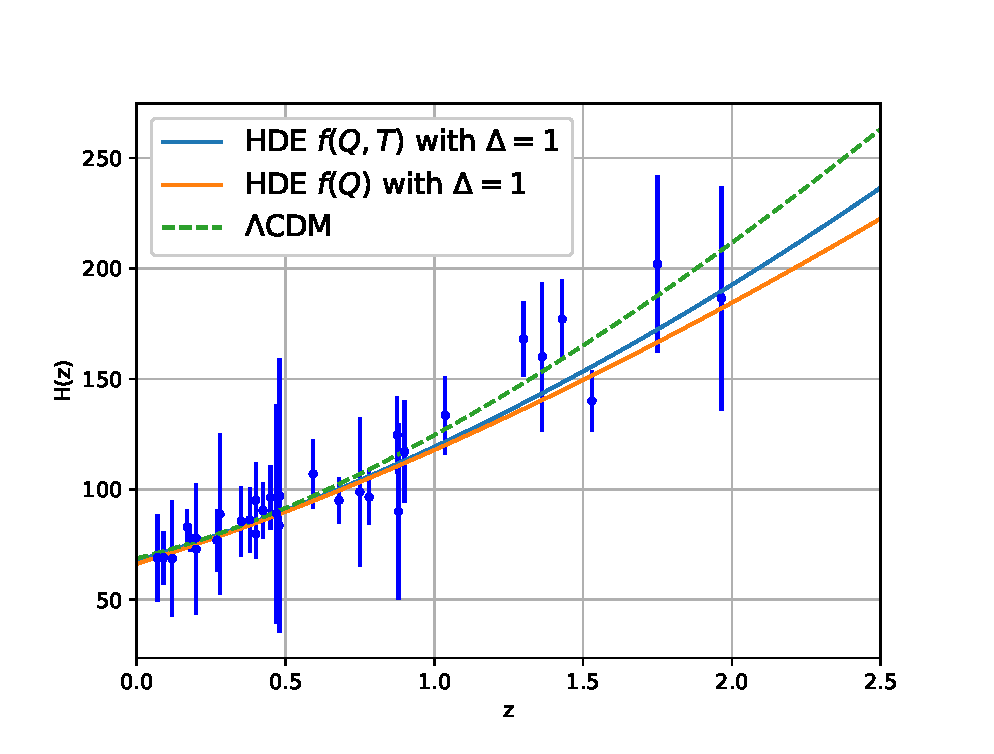
\includegraphics[width=0.45\textwidth]{./pic/H-z_relation.eps}}
    \subfigure[Data points of supernova distance modulus versus redshift along with the best-fit curves for each model.]{
    \label{Fig.sub.2}
    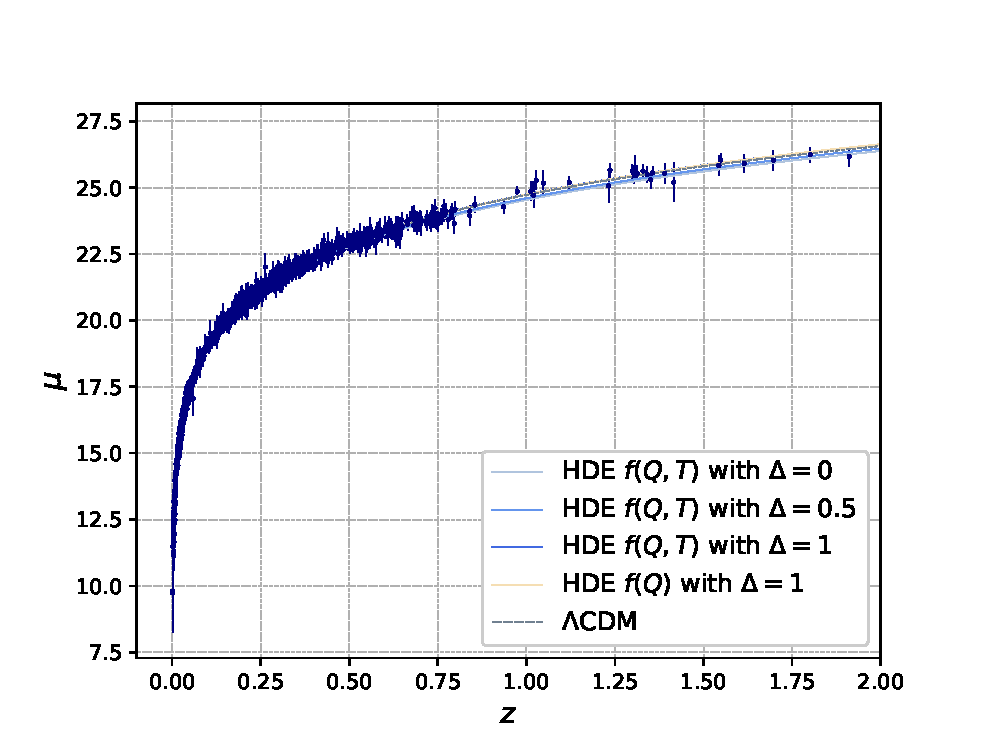
\includegraphics[width=0.45\textwidth]{./pic/mu-z_relation.eps}}
    \caption{Observational data and best-fit curves for different models: (a) Supernova distance modulus versus redshift and (b) Cosmic Chronometer (CC) Hubble parameters versus redshift.}
    \label{Fig.main}
\end{figure}

\begin{figure}[htbp]
    \centering
    \subfigure[Hubble distance over the sound horizon at the drag epoch $D_H/r_d(z)$ as a function of redshift $z$.]{
    \label{Fig2.sub.1}
    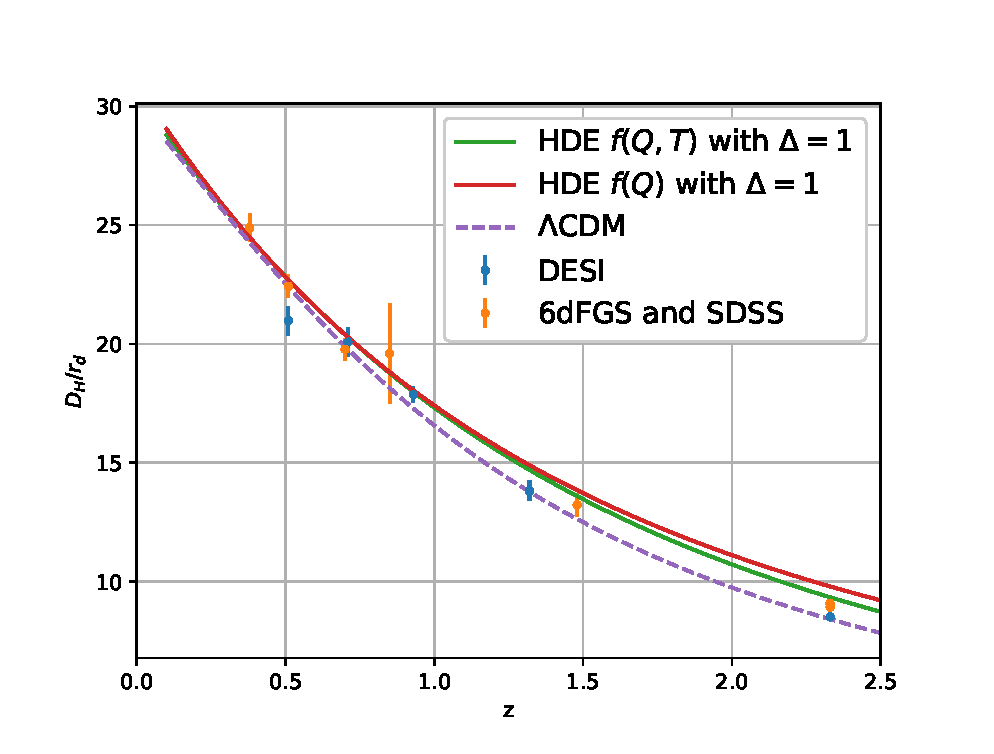
\includegraphics[width=0.45\textwidth]{./pic/DH-z_relation.eps}}
    \subfigure[The comoving diameter distance over the sound horizon at the drag epoch $D_M/r_d(z)$ as a function of redshift $z$.]{
    \label{Fig2.sub.2}
    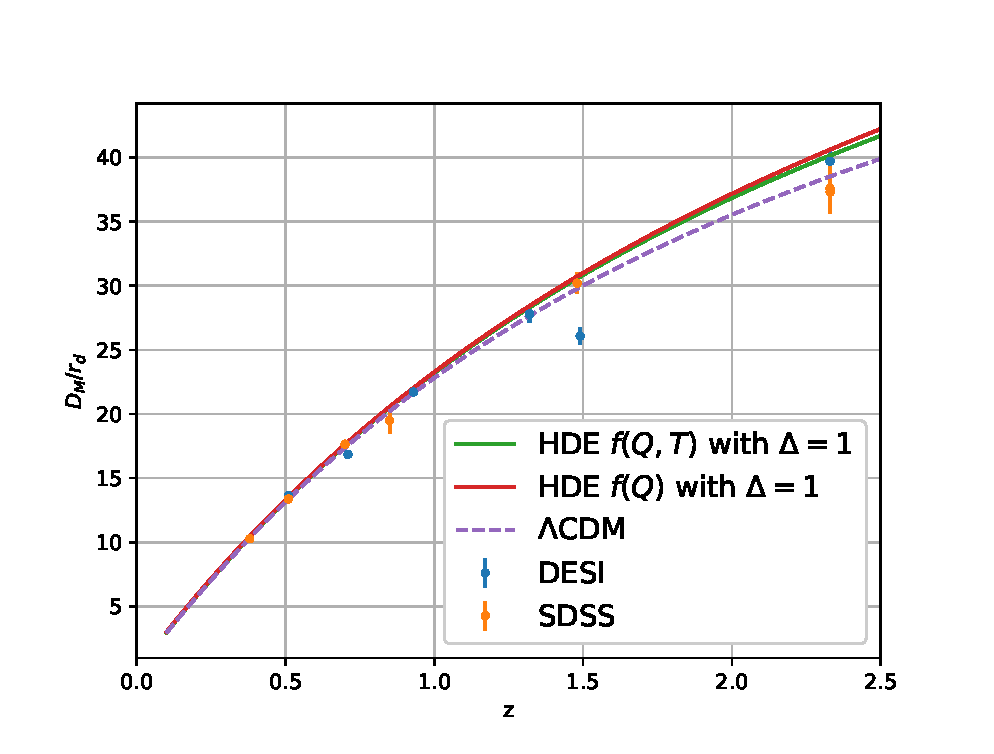
\includegraphics[width=0.45\textwidth]{./pic/DM-z_relation.eps}}
    \subfigure[The angle-average distance over the sound horizon at the drag epoch $D_V/r_d(z)$ as a function of redshift $z$.]{
    \label{Fig2.sub.3}
    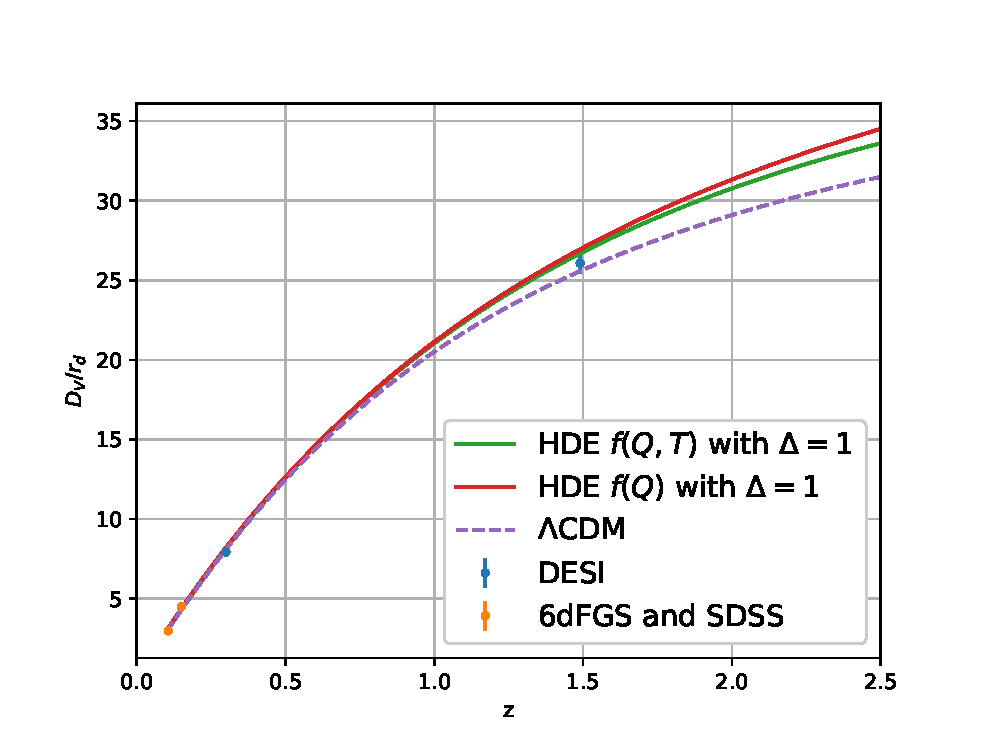
\includegraphics[width=0.45\textwidth]{./pic/DV-z_relation.eps}}
    \caption{Fitting curves of HDE models in BAO, the error bars represent the data from the 6dFGS, SDSS, and DESI BAO measurements.}
    \label{Fig2.main}
\end{figure}

We first plotted the evolution of the Hubble parameter as a function of redshift under the best-fit scenarios for our 4 different models in Fig.~\ref{Fig.sub.1}. For comparison, we also included the evolution curve of the $\Lambda$CDM model under the same conditions. We find that the larger $\Delta$ parameter presents a better fit and gradually reduces the value of the Hubble parameter at high redshifts. We also observe that there is a divergence in whether to consider non-minimum coupling, with minimum coupling models that ignore the interaction tending to present a flatter curve. This phenomenon suggests that the interaction in the non-minimal coupling model redistributes the energy between matter and dark energy, thereby reducing the dominance of matter at high redshift. We also plotted the relationship between the supernova distance modulus predicted by the model and the redshift  (Fig.~\ref{Fig.sub.2}), along with the data points and error lines obtained from the Pantheon+ dataset, and we found that none of the models were significantly different from the fit of the observed supernova distance modulus. The corresponding best fit curve for BAO data with the data points and error lines are also plotted in  Fig.~\ref{Fig2.main}.

\begin{table}[htbp]
    \centering
    \caption{AIC and BIC values for different cosmological models.}
    \begin{tabular}{lcc}
    \toprule
    Model & AIC & BIC \\
    \midrule
    $\Lambda$CDM & 1836.52 & 1858.93 \\
    $f(Q,T), \Delta=0$ & 2204.12 & 2216.71 \\
    $f(Q,T), \Delta=0.5$ & 2091.1 & 2130.31 \\
    $f(Q,T), \Delta=1$ & 1933.97 & 1973.18 \\
    $f(Q), \Delta=1$ & 2056.9 & 2096.11 \\
    \bottomrule
    \end{tabular}
    \label{tab:AICBIC}
\end{table}

We can evaluate the model by calculating the AIC and BIC as shown in Table\ref{tab:AICBIC}. However, it is to be expected that these models deviate significantly from the standard $\Lambda$CDM model. The reasons for the deviation are not only due to the large differences caused by non-metric gravitational forces, but also the coupling effects between geometric tensors and dynamic tensors, which cannot be ignored. More importantly, these models have little cosmological motivation, and it is impossible to restore them to any particular limit case\cite{rudraObservationalConstraintFRT2021}. Nonetheless, the results also show that when $Delta=1$, the dark energy confinement is better than the results in other cases, and that the non-minimally coupled case performs better than the minimally coupled case.

\begin{figure}[htbp]
    \centering
    \subfigure[The evolution of the models' deceleration factor which reflects the accelerating expansion phase in $z\approx 0.8$.]{
    \label{Fig3.sub.1}
    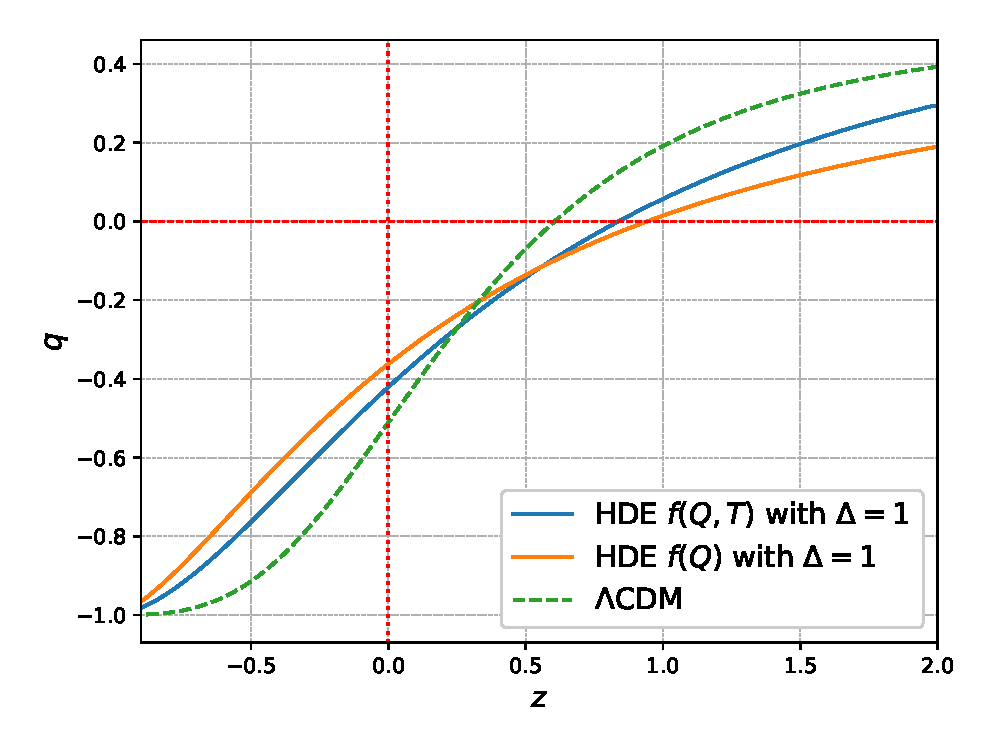
\includegraphics[width=0.45\textwidth]{./pic/q-z_relation.eps}}
    \subfigure[The effective EOS, accounting for all components, provides a direct reflection of the cosmic expansion history and ultimately approaches -1.]{
    \label{Fig3.sub.2}
    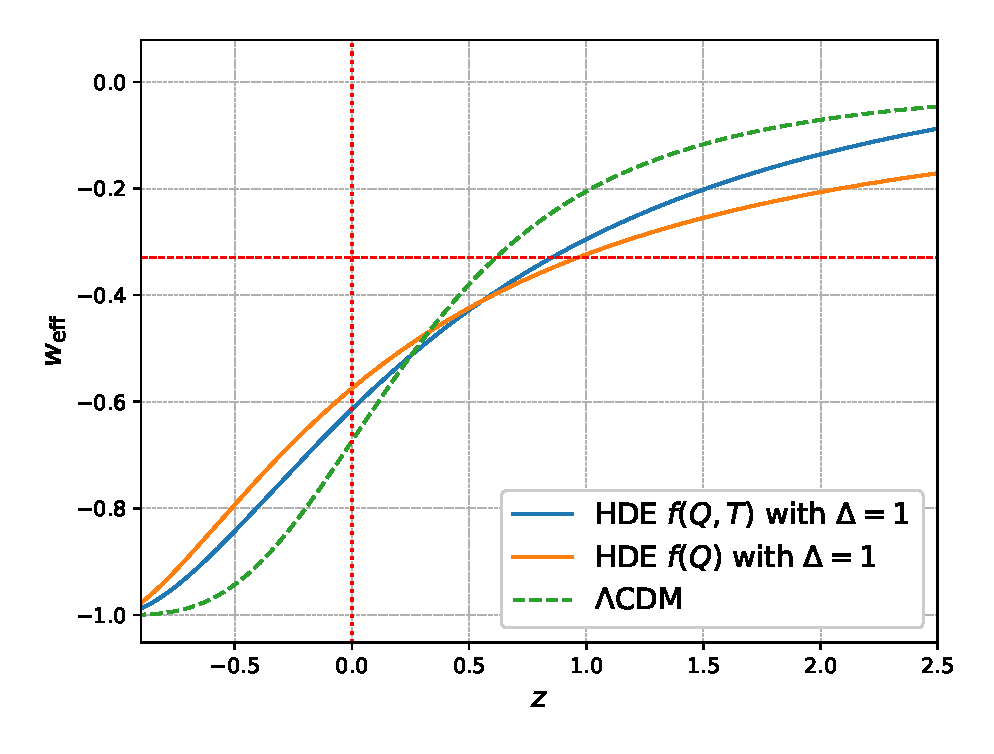
\includegraphics[width=0.45\textwidth]{./pic/w_eff-z_relation.eps}}
    \caption{Evolution of deceleration factor and effective EOS}
    \label{Fig3.main}
\end{figure}

To investigate the evolution of our models, we calculated the deceleration factor and the effective EOS, as shown in Fig. \ref{Fig3.sub.1} and \ref{Fig3.sub.2}. Here we plot only two models of the maximum deformation HDE, because for the other two cases, both parameters are approximately constant and cannot reflect the phase transition and accelerated expansion. We find that the evolution of the deceleration factor for the $\Delta=1$ model reveals a transition to an accelerated expansion phase near $z \approx 0.8$ in accordance with relevant observations. At the same time, effective EOS takes into account all the components of the universe, providing a comprehensive reflection of the expansion history of the universe, and in the future this count approaches $-1$, consistent with the cosmological constant dominating the universe, at the current time is also at $w_\text{eff} \approx -0.6$ reflecting accelerated expansion in our universe.

\section{Conclusion}\label{sec:conclusion}

In this paper, we discuss the evolution of holographic dark energy under the non-metric modified gravity theory $f(Q,T)$. Although this seems to be an overly complex assumption, in fact, if we are in a universe with non-metric geometry (such as Weyl-Cartan geometry) instead of Riemannian geometry, we cannot simply assume that dark energy no longer exists as a fluid in such a universe. We still regard it as one of the reasons for the expansion of the universe, even in such a complex cosmological background.

We also consider holographic dark energy because it has a solid theoretical basis and is a generalization of the holographic principle in cosmology. Holographic dark energy provides a reasonable explanation for the origin of dark energy, namely, it originates from the entanglement entropy of the cosmological horizon. In order to describe holographic dark energy more accurately, we introduce the generalized Barrow holographic dark energy model, which can better characterize quantum corrections. In terms of the choice of infrared cutoff, we use the Hubble horizon as the infrared cutoff point because it is the most natural and simple choice, although other horizons can also be considered. At the same time, in order to facilitate the calculation of analytical solutions, we considered several special cases, namely the loosest restriction when $\Delta=0$, the largest quantum correction when $\Delta=1$, and an intermediate case when $\Delta=0.5$, and discussed whether there is the influence of non-minimum energy-momentum tensor coupling, which makes the interaction between ideal fluid and geometry possible.

To validate the model, we performed parameter estimation using recent supernova data, BAO data, and direct measurements of the Hubble parameter. By employing the MCMC method, we obtained estimates for the model parameters. Our results show that the model can effectively alleviate the Hubble constant tension. Specifically, we find that the Hubble constant is $67.7^{+2.5}_{-2.7}\, \text{km/s/Mpc}$, a deviation greater than 2 $\sigma$ of lastest constraint result of $\Lambda$CDM $69.48^{+0.94}_{-0.94}\, \text{km/s/Mpc}$ through DESI BAO and Planck measurements \cite{pogosian2024consistencytestcosmologicalmodel}. We also study the evolution of the universe under this model and observe that the deceleration factor and the effective EOS parameter indicate accelerated expansion, consistent with current observations.

Among the models we considered, we compared AIC and BIC and found that the best result was obtained when $\Delta=1$, which is the maximum deformation of Bekenstein-Hawking entropy and the more stringent ultraviolet cutoff. We also compared it with the case of minimum coupling and found that considering the coupling of the matter-energy-momentum tensor in the Lagrangian has a better fit to the actual observations despite the addition of the interaction between geometry and matter-energy-momentum tensor.

Although this model is not a convincing consideration, for that it not only introduces too many parameters, and has a large number of assumptions, but we get some interesting results and related analysis and some mathematical conclusions, we are very happy to think in form, and carry out related parameter estimation, which may have some enlightenment on non-metric gravity. Trying to understand the nature of dark energy and the expansion of the universe is still a long-term process.

\section*{Acknowledge}

% Numbered list
% Use the style of numbering in square brackets.
% If nothing is used, default style will be taken.
%\begin{enumerate}[a)]
%\item 
%\item 
%\item 
%\end{enumerate}  

% Unnumbered list
%\begin{itemize}
%\item 
%\item 
%\item 
%\end{itemize}  

% Description list
%\begin{description}
%\item[]
%\item[] 
%\item[] 
%\end{description}  

% \clearpage %%Remove this from your manuscript




% Uncomment and use as the case may be
%\begin{theorem} 
%\end{theorem}

% Uncomment and use as the case may be
%\begin{lemma} 
%\end{lemma}

%% The Appendices part is started with the command \appendix;
%% appendix sections are then done as normal sections
%% \appendix

% To print the credit authorship contribution details
% \printcredits

%% Loading bibliography style file
% \bibliographystyle{elsarticle-num}
% \bibliographystyle{cas-model2-names}

% % Loading bibliography database
% \bibliography{cas-refs}

\printbibliography
% Biography
%\bio{}
% Here goes the biography details.
%\endbio

%\bio{pic1}
% Here goes the biography details.
%\endbio

\end{document}

